% This document is used for Daya Bay MACRO PMT pressure test report


\documentclass{beamer}
\usepackage{graphicx}

\newcommand{\tabincell}[2]{\begin{tabular}{@{}#1@{}}#2\end{tabular}}

\usepackage{ragged2e}
\justifying

\usepackage{setspace}

\setbeamertemplate{navigation symbols}{}
\setbeamertemplate{footline}[page number]
\setbeamertemplate{caption}[numbered]

\usetheme{default}
\logo{
\includegraphics[height=1cm]{Dyb_logo.png}}
\begin{document}
\title{Status of MACRO PMT pressure tests at SAB}
\author{Logan Lebanowski, Shih-Kai Lin}
\institute{University of Houston}
\date{2010 November 18}

\begin{frame}
\begin{center}
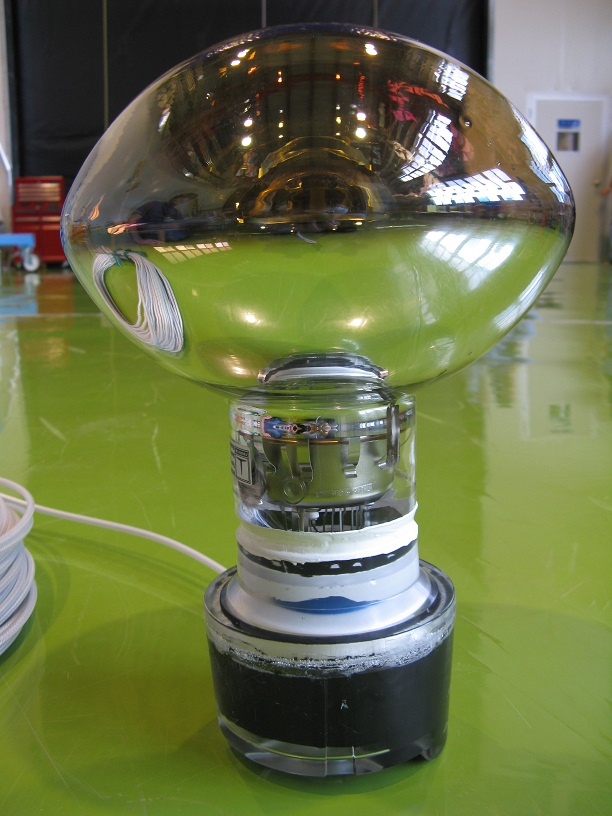
\includegraphics[height=4cm]{IMG_1048.jpg}
\end{center}
\titlepage
\end{frame}


\begin{frame}{overview}
	\begin{itemize}
		\item 150 waterproof MACRO EMI PMT assemblies need to be pressure tested
			at the SAB. They have already passed performance tests at DGUT.
		\item We test about 10 PMTs per week (mid-August to December).
		\item For more information, see
			\textcolor{blue}{\href
			{http://dayabay.ihep.ac.cn/cgi-bin/DocDB/ShowDocument?docid=5373}{doc 5373}}.
	\end{itemize}
		\begin{center}
			\underline{As of November 18, we have passed 97 of 108 tested MACRO PMTs}\\
		\end{center}
	\begin{center}
		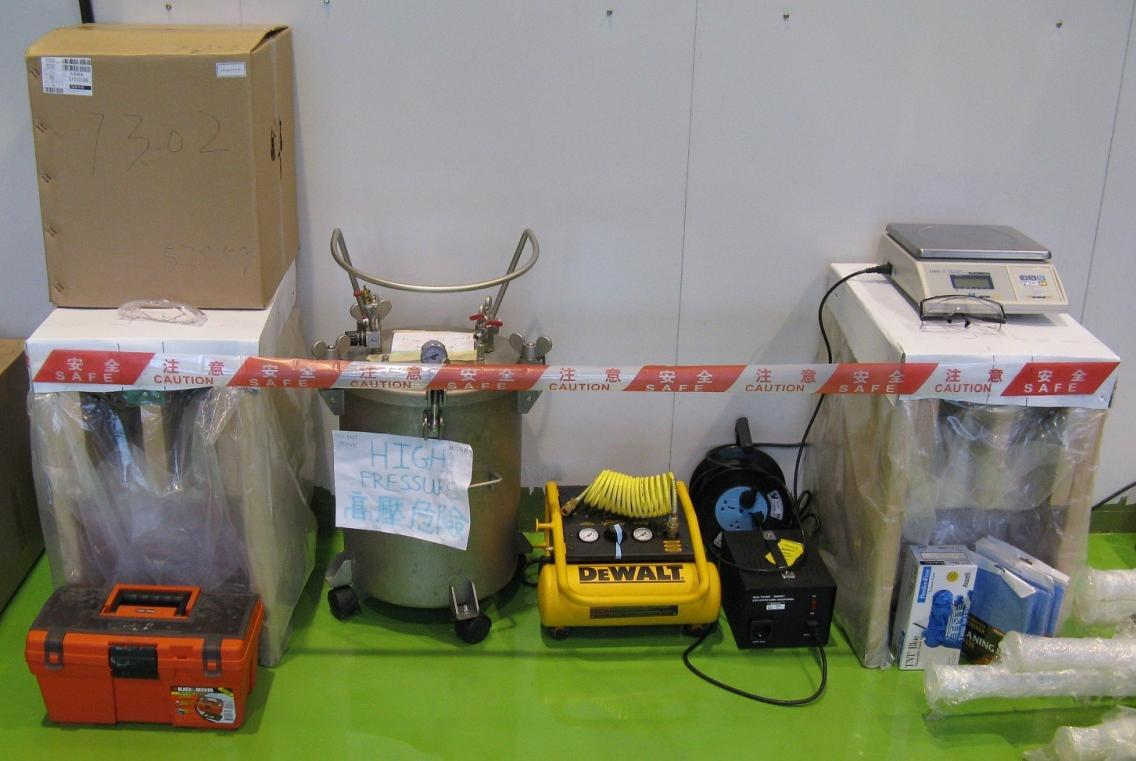
\includegraphics[height=4cm]{test_setup.jpeg}
	\end{center}
\end{frame}


\begin{frame}{pressure test results}
	\begin{center}
		\small
		11 PMTs were tested during the past week (Nov 11 - November 17).
	\end{center}
\begin{table}
\small
\setstretch{0.4}
\begin{tabular}{c|c|c|c|c}
	SN & mass(g) & pressure (psig) & test time (h:m) & result \\
	\hline
	8927 & 3046.5$^\dagger$ & 13.0 & 16:42 & PASS$^2$ \\
	7113 & 3042.5$^\dagger$ & 11.9 & 7:49 & PASS$^1$ \\
	6908 & 589.0 & 12.0 & 15:00 & PASS$^1$ \\
	7727 & 583.5 & 12.0 & 8:13 & PASS$^1$ \\
	7224 & 614.0 & 12.0 & 16:18 & PASS$^2$ \\
	6300 & 608.0 & 12.0 & 46:47 & PASS$^2$ \\
	7660 & 593.5 & 12.0 & 8:18 & PASS$^1$ \\
	6587 & 570.5 & 12.0 & 15:00 & PASS$^1$ \\
	{\color{red}6455} & {\color{red}558.5} & {\color{red}12.2} & {\color{red}$<$8:21}
	& {\color{red}FAIL$^3$} \\
	7739 & 594.0 & 12.1 & 15:20 & PASS$^1$ \\
	7037 & 576.5 & 12.1 & 7:10 & PASS$^1$ \\
\end{tabular}
\end{table}
	\setstretch{0.1}
	\scriptsize
	$^\dagger$ This PMT doesn't have unpotted weight. 12.0 psig of pressure was applied
	according to unpotted-potted mass correlation.\\
	$^1$ Cable dry. No leaks or cracks.\\
	$^2$ 1+Some water penetrated the mastic tape seal of the cable
		strain relief plug, but did not penetrate the UW cable plug.\\
	{\color{red}$^3$ PMT was broken. (see photos in the next page)}
%	$^3$ Cable end sealing tube was full of water. It will be fixed and tested again.

%\begin{itemize}
%	\item For PASS/FAIL reasons, please see the table in the next slide.
%\end{itemize}
%	\setlength{\tabcolsep}{2pt}
%	\tiny
%	\begin{table}
%		\begin{tabular}{|c|p{3.5in}|}
%		\hline
%		1 & Cable dry. No cracks. No leaks detected to within 3.0g
%		    (determined by weighing before and after testing.)\\
%		\hline
%		3 & Cable sealing tube still had some water. The way the cable was repaired didn't
%		work well.\\
%		\hline
%		\end{tabular}
	%\caption{PASS/FAIL reasons}
%	\end{table}
\end{frame}

\begin{frame}{photos: PMT 6455}
	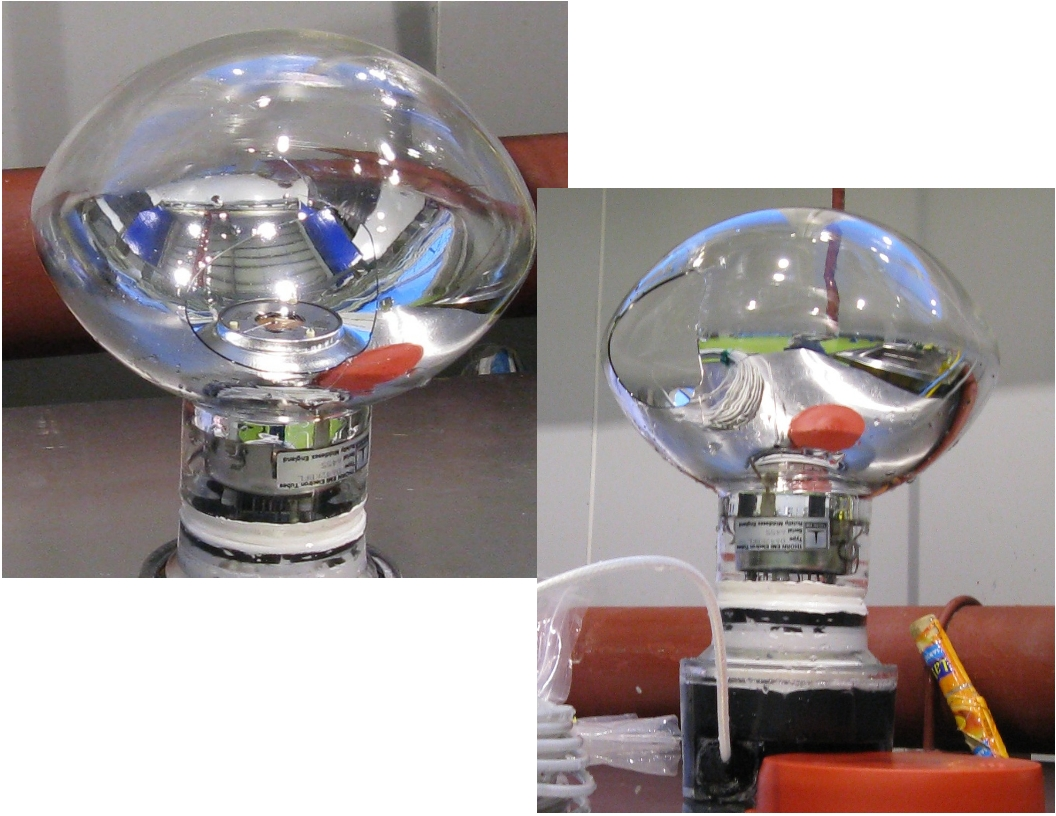
\includegraphics[width=11cm]{PMT6455.jpg}
\end{frame}


\begin{frame}{signal test results}
	\setstretch{0.3}
	\small The operational capability of a PMT is verified after pressure testing:\\
	{\scriptsize The PMT is placed in a dark box, connected to a single channel decoupler box,
	and set to its 2E7 gain voltage, as recorded in the DGUT data. After tens of minutes,
	the count rate, rise time, and pulse height are recorded. We use a threshold of 3.00 
	mV, which is roughly 1/4 pe.
	}

	\setstretch{1}
	\setlength{\tabcolsep}{2pt}
	\scriptsize
	\begin{center}
	\begin{tabular}{|l|p{1.2cm}|p{1.9cm}|p{1.5cm}|p{2.0cm}|}
		\hline
		\textbf{SN}&\textbf{Rate (kHz)}&\textbf{DGUT rate (kHz)}&\textbf{Rise time (ns)}&
		\textbf{DGUT rise time (ns)}\\
		\hline
		\hline
		7961   &3.8&0.47&4.8&4.9\\
		7804   &5.2&0.44&4.9&3.2\\
		6514   &5.3&0.6&4.9&8.2\\
		6477   &12.5$^\dagger$&1.72&5.4&5.1\\
		7415   &7.5&5.29&4.7&6.8\\
		6619   &2.3&0.56&4.7&4.8\\
		7087   &9.5&0.44&5.2&4.3\\
		7199   &7.0&0.4&5.5&4.7\\
		8927   &3.0&0.59&5.5&5.8\\
		7113   &3.0&0.63&5.6&6.6\\
		6908   &1.5&0.36&5.3&5.7\\
		7727   &3.4&0.35&4.2&6.6\\
		7224   &2.0&0.32&5.6&7.8\\
		6300   &1.8&0.5&5.1&6.2\\
		7660   &4.5&0.51&5.5&2.8\\
		\hline
	\end{tabular}
	\scriptsize
		\\$^\dagger$ The rate could be below 10 kHz if it was given enough time.
	\begin{flushleft}
	\end{flushleft}
	\end{center}
\end{frame}

\begin{frame}{PMTs not passed so far}
	\begin{center}
		\begin{table}
			\begin{tabular}{|c|c|}
			\hline
			SN   & reason of failure \\
			\hline
			8430 & crack and hole on photocathode \\
			7046 & imploded \\
			6545 & imploded \\
			6455 & broken \\
			\hline
			\end{tabular}
		\caption{PMTs failed}
		\end{table}

		\begin{table}
			\begin{tabular}{|c|c|}
			\hline
			SN   & reason of not pass \\
			\hline
			8727 & hole in cable jacket \\
			7368 & water leaks into acrylic shell cap \\
			7934 & water leaks into acrylic shell cap \\
			8870 & hole in cable jacket \\
			7343 & water leaks into acrylic shell cap \\
			8377 & hole in cable jacket \\
			7130 & hole in cable jacket \\
			\hline
			\end{tabular}
		\caption{PMTs not passed}
		\end{table}
	\end{center}
\end{frame}

\end{document}